\section{Entwurf}\label{entwurf}
\subsection{Format/Kompotenzmodell}

Für die Modellierung der Kompetenzen gibt es mehrere Möglichkeiten. 

\subsubsection{ESCO RDF Import}

ESCO steht als RDF Graph zur mit einem eigenen Vokabular zur Verfügung und kann mittels RDF Importer\todo{Jesus Barrasa zitieren} in die Neo4j Instanz geladen werden. Dabei werden nach den ESCO Ontologien folgende interessante Knoten und Beziehungstypen angelegt. 

ESCO concepts Relationship

IRI: http://data.europa.eu/esco/modelRelationship


Beziehung zwischen zwei ESCO Säulen tb. Occupation und Qualification.

Qualification 

IRI: http://data.europa.eu/esco/modelQualification

Ein offiziell oder formelles Zertifikat eines oder mehrerer Kompetenzen oder Fertigkeiten.

Kann verknüpft im Skills oder Berufen sein.

Skil 

IRI: http://data.europa.eu/esco/modelSkill


\todo{weitere auf https://ec.europa.eu/esco/resources/data/static/model/html/model.xhtml }

\subsubsection{inLOC}

Das Projekt InLOC ermöglicht das Abbilden von allen Kompetenzrahmen in einem einheitlichen maschienenlesbaren Format(RDF,XML,JSON-LD).


\subsubsection{Datenbank}

Für die Persistenz der Kompetenz Daten wird eine Instanz des Neo4j Datenbank Management Systems eingesetzt. Die Vorteile 

Alternative Datenbanken
Warum keine RDF Technologie?
\subsubsection{API}

 Die Funktionsweise der Recommendation Engine soll sich lediglich auf folgende Prozesse beschränken:
 
 Eingabe und Ausgabe einer Kompetenz
Berechnung von Ähnlichkeiten im Graphen durch Graph Traversierung

Die Anwendung ist also wenig Komplex. Ein viel höherer Implementierungsaufwand ist den Vergleichsalgorithmen, bzw Graph Queries zuzurechnen. Um den Implementierungsaufwand der Applikation weiter zu reduzieren, soll das Serverless Framework für Amazon Web Services Lambda zum Einsatz kommen. 

Für die erste Komponente wird eine Web Api benötigt, über welche  mit einem Internetfähigen Protokoll wie zb. HTTP zugegriffen werden kann. 

Die Zweite Komponente muss eine Datenbankanbindung für die Datenbank gewährleisten, und Daten aus der Eingabe in Anfragen an die Datenbank verarbeiten, sowie Ergebnisse der Anfragen zurückliefern. Falls die Anfragensprache der Datenbank nicht alle Möglichkeiten ausschöpfen kann die Ergebnisse wie gewünscht zu filtern, können in der zweiten Komponente weitere Algorithmen implementiert werden.


\begin{figure}[htb]
 \centering
 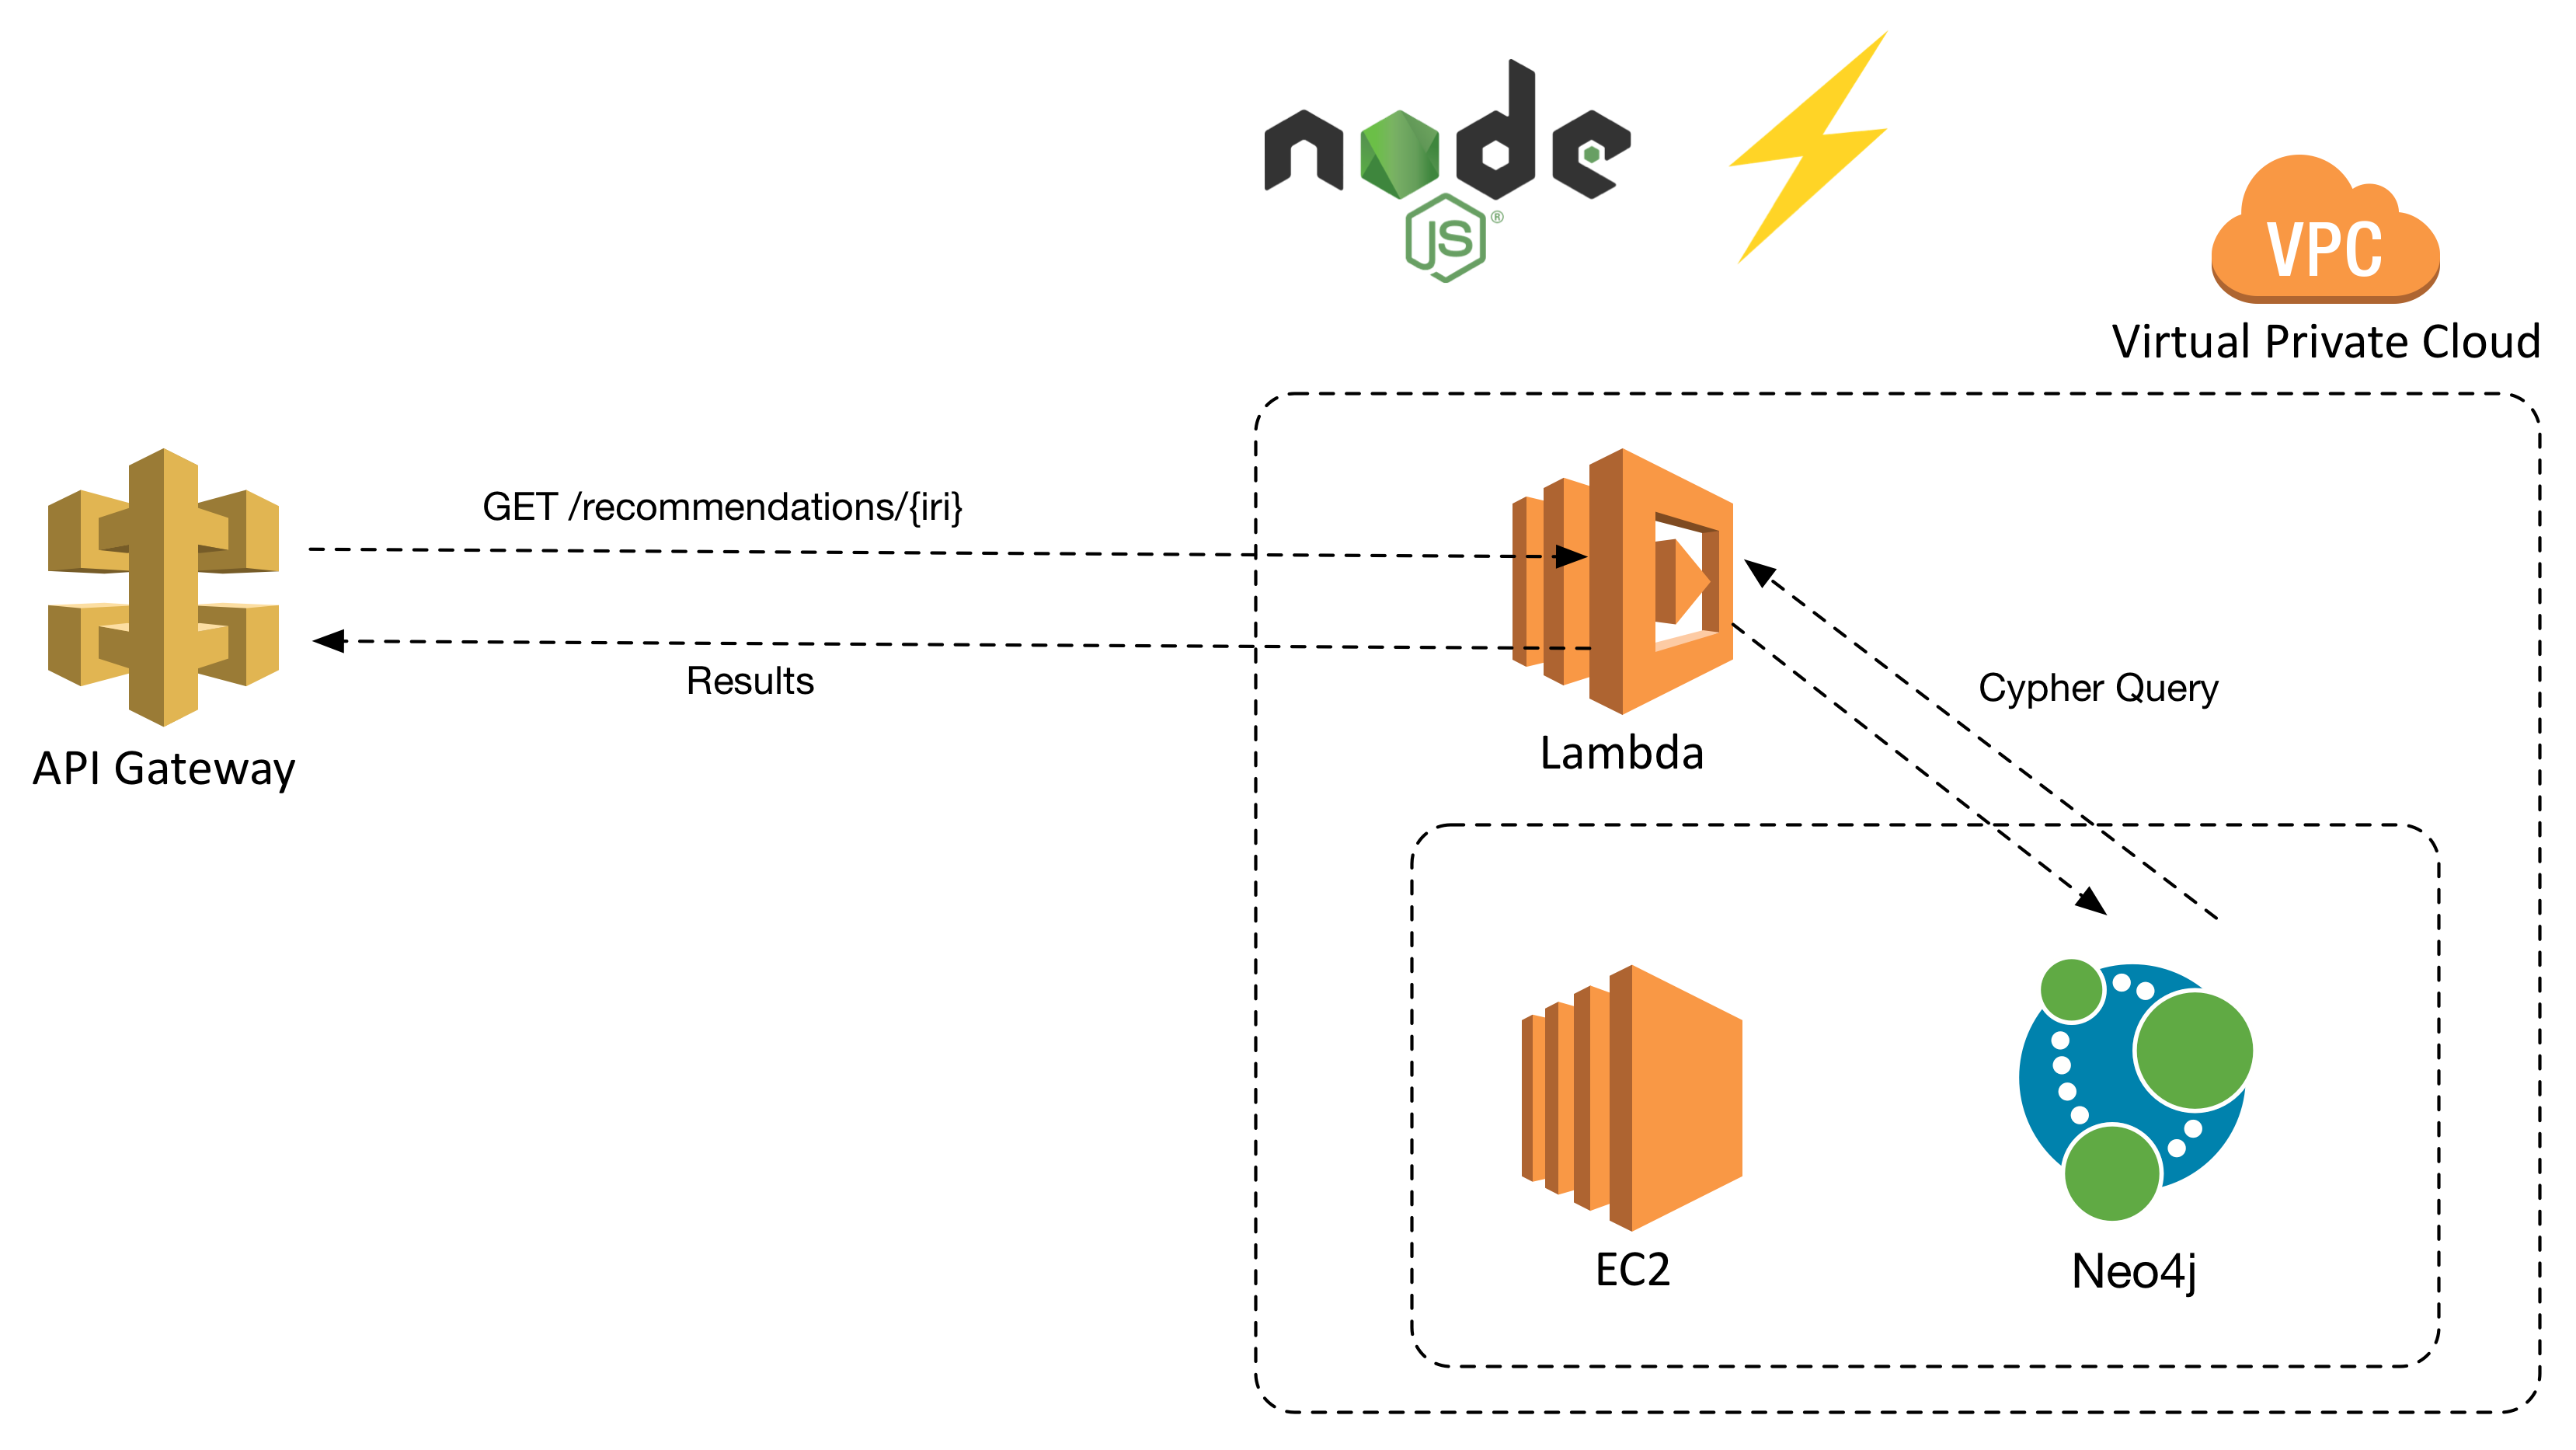
\includegraphics[width=0.7\textwidth,angle=0]{abb/Architecture}
 \caption[Beschreibung]{Beschreibung}
\label{fig:Beschreibung}
\end{figure}

\subsection{Datenmodell}
\subsection{Anfragen Formulieren}
\subsection{Algorithmen}

Shortest Path
Dijkstra Algorithm
Depth First
Breadth first search
